
\subsection{Soluzioni di esercizi nella sezione ``\textbf{\nameref{subsec:the:circle}}"}

% https://math.libretexts.org/Courses/Monroe_Community_College/MTH_165_College_Algebra_MTH_175_Precalculus/03%3A_Polynomial_and_Rational_Functions/3.02%3A_Circles/3.2e%3A_Circle_Exercises.
% https://math.libretexts.org/Courses/Monroe_Community_College/MTH_165_College_Algebra_MTH_175_Precalculus/03%3A_Polynomial_and_Rational_Functions/3.02%3A_Circles/3.2e%3A_Circle_Exercises.

Soluzione dell'esercizio \ref{circ_00} a pagina \pageref{circ_00}\label{circs_00}

\[
(x-8)^2+(y+10)^2=64
\]

\vspace{1cm}
\hrule
\vspace{1cm}


Soluzione dell'esercizio \ref{circ_01} a pagina \pageref{circ_01}\label{circs_01}

Center: $(2,1)$

Radius: $r=2$
\[
(x-2)^2+(y+1)^2=4
\]

\vspace{1cm}
\hrule
\vspace{1cm}


Soluzione dell'esercizio \ref{circ_02} a pagina \pageref{circ_02}\label{circs_02}

Center: $(-1,3)$

Radius:  $r=5$

\[
(x+1)^2+(y-3)^2=25  
\]

\vspace{1cm}
\hrule
\vspace{1cm}


Soluzione dell'esercizio \ref{circ_03} a pagina \pageref{circ_03}\label{circs_03}

\begin{itemize}
\item[a] Center $(2,-3)$, radius  $r=3$
\item[b] Center $(2,-5)$, radius  $r=2$
\item[c] Center $(-9,0)$, radius  $r=5$
\item[d] Center $(-\frac{1}{2},\frac{3}{5})$, radius  $r=\frac{\sqrt{161}}{10}$
\end{itemize}


\begin{figure}[H]
\centering
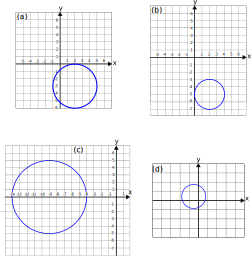
\includegraphics[width=0.9\textwidth]{circles_02.pdf}
\end{figure}




\vspace{1cm}
\hrule
\vspace{1cm}


Soluzione dell'esercizio \ref{circ_04} a pagina \pageref{circ_04}\label{circs_04}

\vspace{1cm}

Bisogna riscrivere l'equazione 

\[
x^2+y^2-6x+8y+24=0 
\]

nella forma dell'equazione standard del cerhio (l'equazione \ref{cerchio:equazione} a pagina \pageref{cerchio:equazione}):


\[
(x-h)^2+(y-k)^2=r^2
\]

Per fare ciò, spostiamo i termini variabili alla sinistra e le costanti a destra del segno di uguaglianza, e concentriamo l'attenzione sui termini con la $x$:

\begin{equation} \label{circ:04:1}
\underline{x^2-6x}+y^2+8y=-24
\end{equation}

Ora teniamo bene a mente come è fatto il quadrato del binomio:

\[
(x-h)^2 = x^2-2hx +h^2
\]

Guardando bene i termini con la $x$ nell'espressione \ref{circ:04:1}, troveremo che quel $-6x$ somiglia molto a $2\times -3\times x$, quindi basterebbe avere un $9$ per poter costruire un perfettamente plausibile quadrato: $x^2-6x+9$, il che ci direbbe che $h=-3$.

Possiamo aggiungere $9$ ad entrambi i termini dell'uguaglianza:


\[
\underline{x^2
-6x
+9
}
+y^2
+8y=-24 + 9 
\]

Ora possiamo raggruppare $x$:


\[
\underline{(x-3)^2 }
+y^2
+8y=-24 + 9 
\]

Facciamo lo stesso giochino con le $y$ , in quanto $+8y$ è $2\times 4 \times y$ quindi aggiungiamo $16$ da entrambe le parti come abbiamo fatto prima:

\[
(x-3)^2 
+y^2
+8y
+16
=-24 + 9 +16
\]

Ora l'equazione diventa:

\[
(x-3)^2+ 
(x+4)^2
=1
\]


Abbiamo quindi trovato i valori che ci serviuvano e cioè $h=3$, $k=-4$, $r=1$.

In altre parole il nostro cerchio ha il centro in $(3,-4)$ e un raggio pari a $1$.



\vspace{1cm}
\hrule
\vspace{1cm}


Soluzione dell'esercizio \ref{geop_01} a pagina \pageref{geop_01}\label{geos_01}

The tangent(s) are of the form $y = mx + 14$ because they go through $(0,14)$.

Substitute this into the equation of the circle:


\[
x^2+y^2+14x-6y=-41
\]

\[
x^2+(mx+14)^2+14x-6(mx+14)+41=0
\]


\[
x^2+m^2x^2+28mx+196+14x-6mx-43=0
\]

\[
(1+m^2)x^2+(22m+14)x+153=0
\]

This is a quadratic equation: $ax^2+bx+c=0$
where
\begin{enumerate}
\item $a=1+m^2$
\item $b=22m+14$
\item $c=153$
\end{enumerate}

The discriminant ($b^2-4ac$) tells us how many solutions does the equation have.

In this case we are looking for a single solution because the lines are tangent to the circle, i.e. each line touches the circle in one point only.

So the discriminant (often written as $\Delta$) must be zero:

\[
(22m+14)^2-4(1+m^2)153=0
\]

\[
484m^2+616m+196-612-612m^2=0
\]

\[
-128m^2+616m-416=0
\]

Now this is a simple quadratic equation, let's apply the formula:

\[
m=\frac{-b\pm\sqrt{b^2-4ac}}{2a}=\frac{-616\pm \sqrt{616^2-4\times(-128)\times(-416)}}{2\times -128}
\]


\[
m=\frac{-616\pm \sqrt{379456-212992}}{-256}
\]


\[
m=\frac{-616\pm 408}{-256}
\]

\[
\left\{
\begin{array}{ll}
m_1=\frac{-616+408}{-256}=\frac{-208}{-256}=\frac{13}{16}\\
\\
m_2=\frac{-616-408}{-256}=4
\end{array}
\right.
\]

\[
\left\{
\begin{array}{ll}
l_1: y=\frac{13}{16}x+14\\
\\
l_2: y=4x+14
\end{array}
\right.
\]

\vspace{1cm}
\hrule
\vspace{1cm}


Soluzione dell'esercizio \ref{circ_06} a pagina \pageref{circ_06}\label{circs_06}

È necessario per prima cosa riscrivere le equazioni nella seguente forma:

\[
(x-h)^2+(y-k)^=r^2
\]

dove 
\begin{itemize}
\item[\textbf{h}] è la coordinata $x$ del centro
\item[\textbf{k}] è la coordinata $y$ del centro
\item[\textbf{r}] è il raggio
\end{itemize}

Raccogliendo per $x$ e $y$ otteniamo: 

\[
\begin{split}
(a): (x^2-2x)+(y^2-4y)=4 \\
\\
(b): (x^2-4x)+(y^2-2y)=-4
\end{split}
\]

Facendo riferimento per ora alla sola equazione $(a)$, per trasformare
i termini $(x^2-2x)$ e $(y^2-4y)$ nella forma $(x-h)^2, (y-k)^2$ dobbiamo
seguire per ognuno dei termini questi passi:

\begin{enumerate}
\item considerare il coefficiente del termine di primo grado
\item dividere per $2$
\item calcolarne il quadrato
\item aggiungere il risultato da entrambi i lati dell'equazione
\end{enumerate}

Questo significa che per il termine $(x^2-2x)$ avremo:

\begin{enumerate}
\item il coefficiente del termine di primo grado è $2$
\item $2/2=1$
\item $1^2=1$
\item aggiungere questo risultato a entrambi i lati dell'equazione, che diventa:
\[
(a): (x^2-2x+1)+(y^2-4y)=4+1
\]
\end{enumerate}

Per il termine $(y^2-4y)$ avremo che:
\begin{enumerate}
\item il coefficiente del termine di primo grado è $4$
\item $4/2=2$
\item $2^2=4$
\item aggiungere il risultato a entrambi i lati dell'equazione, che diventa:
\[
(a): (x^2-2x+1)+(y^2-4y+4)=4+1+4
\]
\end{enumerate}

A questo punto possiamo riscrivere l'equazione come segue:

\[
(a) (x-1)^2+(y-2)^2=3^2
\]

Quindi la prima circonferenza avrà il centro in $(1, 2)$ e raggio 3.

Allo stesso modo la seconda equazione potrà essere riscritta come segue:
\[
(b) (x-2)^2+(y-1)^2=1
\]

Quindi la seconda circonferenza avrà il centro in $(2, 1)$ e raggio 1.

Un veloce grafico ci dirà che la soluzione esatta è la $B$:
le due circonferenze sono disgiunte e la seconda è interna alla prima.

\begin{figure}[H]
\centering
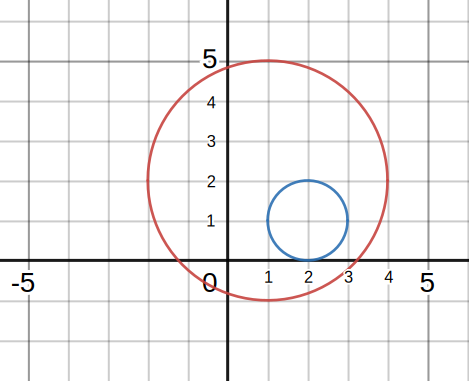
\includegraphics[width=0.6\textwidth]{circ_06.pdf}
\end{figure}

N.B.: la risposta $D$ era comunque da scartare in quanto due circonferenze
possono avere solo zero punti in comune (disgiunte) oppure un
punto in comune (tangenti) oppure due punti in comune (intersecanti),
oppure infiniti punti in comune (identiche e sovrapposte).



\vspace{1cm}
\hrule
\vspace{1cm}


Soluzione dell'esercizio \ref{circ_07} a pagina \pageref{circ_07}\label{circs_07}

Congiungendo i centri dei cerchi si ottiene un triangolo equilatero di lato $k=2$.


\begin{figure}[H]
\centering
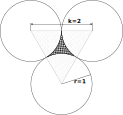
\includegraphics[width=0.6\textwidth]{circles04.pdf}
\end{figure}

L'altezza del triangolo è \[\sqrt{2^2-1^2}=\sqrt{3}\]
La sua area è \[\frac{2\cdot\sqrt{3}}{2}=\sqrt{3}\]
L'area del cerchio di raggio $1$ è $\pi$.

La parte tratteggiata a puntini consiste di tre settori circolari,
ognuno di area $\frac{\pi}{6}$.

La risposta al problema è quindi \[\sqrt{3}-3\frac{\pi}{6}=\sqrt{3}-\frac{\pi}{2}\]


\vspace{1cm}
\hrule
\vspace{1cm}


 Soluzione dell'esercizio \ref{circ_08} a pagina \pageref{circ_08}\label{circs_08}

Trovare l'area della parte tratteggiata in grigio:

\begin{figure}[H]
\centering
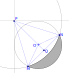
\includegraphics[width=0.6\textwidth]{circ_07.pdf}
\end{figure}



L'area da calcolare ($i$) consiste della differenza tra i due segmenti circolari
$h$ e $g$, uno sotteso al cerchio grande $a$ e l'altro sotteso al cerchio
piccolo $b$.

Ognuno dei segmenti circolari $h$ e $g$ può essere calcolato come la 
differenza tra il corrispondente settore circolare (``$c$'' e ``$d$'') e 
il triangolo isoscele definito da esso (``$e$'' e ``$f$'').

\begin{figure}[H]
\centering
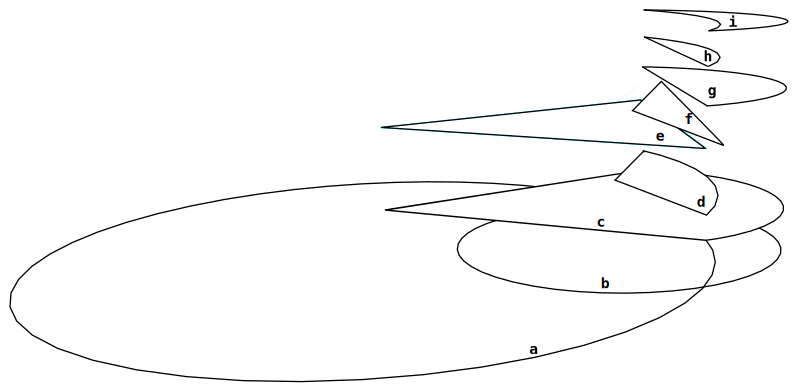
\includegraphics[width=0.9\textwidth]{circles.7.b.pdf}
\caption{Denominazioni dei vari elementi}
\label{fig:denom}
\end{figure}



\begin{figure}[H]
\centering

\includegraphics[width=0.6\textwidth]{circ_07_01.pdf}
\end{figure}


\begin{figure}[H]
\centering
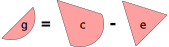
\includegraphics[width=0.6\textwidth]{circ_07_02.pdf}

\includegraphics[width=0.6\textwidth]{circ_07_03.pdf}
\end{figure}

Prima di tutto è necessario calcolare la lunghezza del 
segmento $MN$ definito dai punti di intersezione dei due cerchi.

Sono possibili due soluzioni, una analitica e una geometrica.

La soluzione analitica prevede l'utilizzo 
dell'equazione del cerchio:

\[ (x-h)^2+(y-x)^2=r^2 \]

I due due cerchi in oggetto sono definiti dalle seguenti equazioni:
\[ x^2+y^2=4 \]
\[ (x-1)^2+(y+1)^2=1 \]

Per trovare le coordinate dei punti $M$ e $N$ 
bisogna risolvere un sistema:

\[
\left\{
\begin{array}{ll}
x^2+y^2=4 \\
(x-1)^2+(y+1)^2=1
\end{array}
\right.
\]

La seconda equazione diventa:

\[ x^2 -2x +1 +y^2 +2y+1=1 \]

sostituisco $x^2+y^2$ con $4$:

\[ 4-2x+1+2y=0 \]
\[ 2y=2x-5  \]
\[ y=x-\frac{5}{2} \]

Sostituisco questo $y$ nella prima equazione:

\[ x^2+\left( x-\frac{5}{2} \right)^2=4 \]
\[ x^2+x^2-5x+\frac{25}{4} =4 \]
\[ 2x^2-5x+\frac{9}{4}=0 \]

\[ x=\frac{-b\pm \sqrt{b^2-4ac}}{2a} =
\frac{5\pm \sqrt{5^2-4\cdot 2 \cdot \frac{9}{4}}}{2\cdot 2}\]
\[=\frac{5\pm\sqrt{25-\frac{72}{4}}}{4}
=\frac{5\pm\sqrt{\frac{100}{4}-\frac{72}{4}}}{4}
=\frac{5\pm\sqrt{\frac{28}{4}}}{4}
=\frac{5\pm\sqrt{7}}{4}
\]
\[x_1=\frac{5+\sqrt{7}}{4}
,
x_2=\frac{5-\sqrt{7}}{4}
\]

Ora è possibile calcolare le coordinate $y$ dei punti 
di intersezione:

\[ y=x-\frac{5}{2} \]
\[ y_1=\frac{5+\sqrt{7}}{4}-\frac{5}{2}
, 
y_2=\frac{5-\sqrt{7}}{4}-\frac{5}{2}\]

La lunghezza $L$ della corda $MN$ sarà data da:

\[ L= \sqrt{(x_1-x_2)^2+(y_1-y_2)^2} \]
\[ =\sqrt
{
\left(\frac{5+\sqrt{7}}{4}-\frac{5-\sqrt{7}}{4}\right)^2 +
\left(
	\left( \frac{5+\sqrt{7}}{4}-\frac{5}{2} \right)
	-
	\left( \frac{5-\sqrt{7}}{4}-\frac{5}{2} \right)
\right)^2
} \]

\[ \sqrt{ \left( \frac{2\sqrt{7}}{4} \right)^2 + \left( \frac{2\sqrt{7}}{4} \right)^2} \]

\[ \sqrt { \frac{7}{4} + \frac{7}{4} } = \sqrt{\frac{7}{2}}\]

La formula per l'area del settore circolare è:
\[A=\frac{L\cdot r}{2}\]
dove $L$ è la lunghezza della corda $MN$ e $r$ è il raggio
del cerchio.

L'area del settore circolare del cerchio grande ($P, M, N$) è:
\[A_1=\frac{L\cdot 2}{2}=L\]
mentre quella del cerchio piccolo ($O, M, N$) è
\[A_2=\frac{L\cdot 1}{2}=\frac{L}{2}\]

La formula di Erone permette di calcolare l'area di un triangolo conoscendo
la misura dei lati:

\[A=\sqrt{
\frac{p}{2}
\cdot\left(\frac{p}{2}-a\right)
\cdot\left(\frac{p}{2}-b\right)
\cdot\left(\frac{p}{2}-c\right)
}\]

dove $p$ è il perimetro e $a, b, c$ sono le misure dei tre lati.

Il triangolo 
definito dai punti $P, M, N$
( chiamato $\triangle e$ nella figura \ref{fig:denom} )

avrà quindi area pari a 

\[A_{e}=\sqrt{
\frac{4+L}{2}
\cdot\left(\frac{4+L}{2}-L\right)
\cdot\left(\frac{4+L}{2}-2\right)
\cdot\left(\frac{4+L}{2}-2\right)
}\]
\[=\sqrt{
\frac{4+L}{2}
\cdot\left(\frac{4-L}{2}\right)
\cdot\left(\frac{L}{2}\right)
\cdot\left(\frac{L}{2}\right)
}
=\sqrt{
\frac{
(4+L)(4-L)L^2
}{2^4}
}\]
\[=\frac{L}{4}\sqrt{(4+L)(4-L)}\]

mentre il triangolo definito dai punti $O, N, M$
( chiamato $\triangle f$ nella figura \ref{fig:denom} )
avrà area pari a 


\[A_{t2}=\sqrt{
\frac{2+L}{2}
\cdot\left(\frac{2+L}{2}-L\right)
\cdot\left(\frac{2+L}{2}-1\right)
\cdot\left(\frac{2+L}{2}-1\right)
}\]
\[=\sqrt{
\frac{2+L}{2}
\cdot
\frac{2-L}{2}
\cdot
\frac{L}{2}
\cdot
\frac{L}{2}
}
=\sqrt{
\frac{
(2+L)(2-L)L^2
}{2^4}
}
\]
\[
=\frac{L}{4}
\sqrt{(2+L)(2-L)}
\]

A questo punto è possibile calcolare l'area del segmento circolare 
definito dalla corda $MN$ sul cerchio grande
( chiamato $g$ in figura \ref{fig:denom} ) 
come differenza tra l'area del corrispettivo settore circolare ($c$)
e il triangolo $\triangle e$:
\[  A_g= A_c - A_{\triangle e} \]
\[=L-\frac{L}{4}\sqrt{(4+L)(4-L)}\]

Allo stesso modo si calcola l'area del segmento circolare $h$
definito sul cerchio piccolo come 
\[A_{h}=A_d-A_{\triangle f}\]
\[=\frac{L}{2}-\frac{L}{4}
\sqrt{(2+L)(2-L)}\]

La risposta al quesito dell'esercizio consiste nella differenza tra queste due aree:
\[A_{g}-A_{h}\]
\[=L-\frac{L}{4}\sqrt{(4+L)(4-L)}-\left(\frac{L}{2}-\frac{L}{4}
\sqrt{(2+L)(2-L)}\right)\]

basta sostituire $L$ con il valore trovato precedentemente,
$L=\sqrt{\frac{7}{2}}$:

\[A_{g}-A_{h}\]
\[
=L
-L\frac{1}{4}\sqrt{(4+L)(4-L)}
-\left(L\frac{1}{2}
-L\frac{1}{4}\sqrt{(2+L)(2-L)}\right)
\]

\[
=\sqrt{\frac{7}{2}}
-\frac{1}{4}\sqrt{\frac{7}{2}}\sqrt{\left(4+\sqrt{\frac{7}{2}}\right)\left(4-\sqrt{\frac{7}{2}}\right)}
-\left(\frac{1}{2}\sqrt{\frac{7}{2}}
-\frac{1}{4}\sqrt{\frac{7}{2}}\sqrt{\left(2+\sqrt{\frac{7}{2}}\right)\left(2-\sqrt{\frac{7}{2}}\right)}\right)
\]


\[
=\sqrt{\frac{7}{2}}
-\frac{1}{4}\sqrt{\frac{7}{2}}
\sqrt{\left(16+\frac{7}{2}\right)}
-\frac{1}{2}\sqrt{\frac{7}{2}}
+\frac{1}{4}\sqrt{\frac{7}{2}}\sqrt{\left(4+\frac{7}{2}\right)}
\]

\[
=\sqrt{\frac{7}{2}}\cdot\left(
1-\frac{1}{4}
\sqrt{\frac{39}{2}}
-\frac{1}{2}
+\frac{1}{4}\sqrt{\frac{15}{2}}
\right)
\]

\[
=\sqrt{\frac{7}{2}}\cdot\left(
\frac{1}{2}
-
\frac{\sqrt{39}+\sqrt{15}}{4\sqrt{2}}
\right)
\]

La soluzione geometrica si basa sul fatto che il triangolo 
$\triangle PQM$ è retto, così come lo è $\triangle OQM$. 

Possiamo quindi scrivere che 

\[
\left\{
\begin{array}{ll}
PM^2=QM^2+PQ^2
\\
OM^2=QM^2+OQ^2
\end{array}
\right.
\]

\[
\left\{
\begin{array}{ll}
QM^2=PM^2-PQ^2
\\
QM^2=OM^2-OQ^2
\end{array}
\right.
\]

\[PM^2-PQ^2=OM^2-OQ^2\]

Sappiamo inoltre che
\begin{enumerate}
\item $PQ=OP+OQ$
\item $PM=2$
\item $OM=1$
\item $OP=\sqrt{2}$ essendo il punto $O$ alle coordinate $(1,-1)$
\end{enumerate}



\[4-(\sqrt{2}+OQ)^2=1-OQ^2\]
\[4-2-2\sqrt{2}OQ-OQ^2=1-OQ^2\]
\[-2\sqrt{2}OQ+1=0\]
\[OQ=\frac{1}{2\sqrt{2}}\]
Ora siccome $\triangle MOQ$ è retto:
\[MQ^2=OM^2-OQ^2\]
\[MQ^2=1-\left(\frac{1}{2\sqrt{2}}\right)^2\]
\[MQ^2=1-\frac{1}{8}\]
\[MQ=\sqrt{\frac{7}{8}}\]
\[MN=2\sqrt{\frac{7}{8}}=\sqrt{\frac{28}{8}}\]
\[=\sqrt{\frac{7}{2}}\]

I calcoli di seguito sono identici al caso precedente.



\vspace{1cm}
\hrule
\vspace{1cm}


Soluzione dell'esercizio \ref{circ_09} a pagina \pageref{circ_09}\label{circs_09}

\vspace{1cm}
\hrule
\vspace{1cm}


Soluzione dell'esercizio \ref{circ_10} a pagina \pageref{circ_10}\label{circs_10}

\begin{figure}[H]
\centering
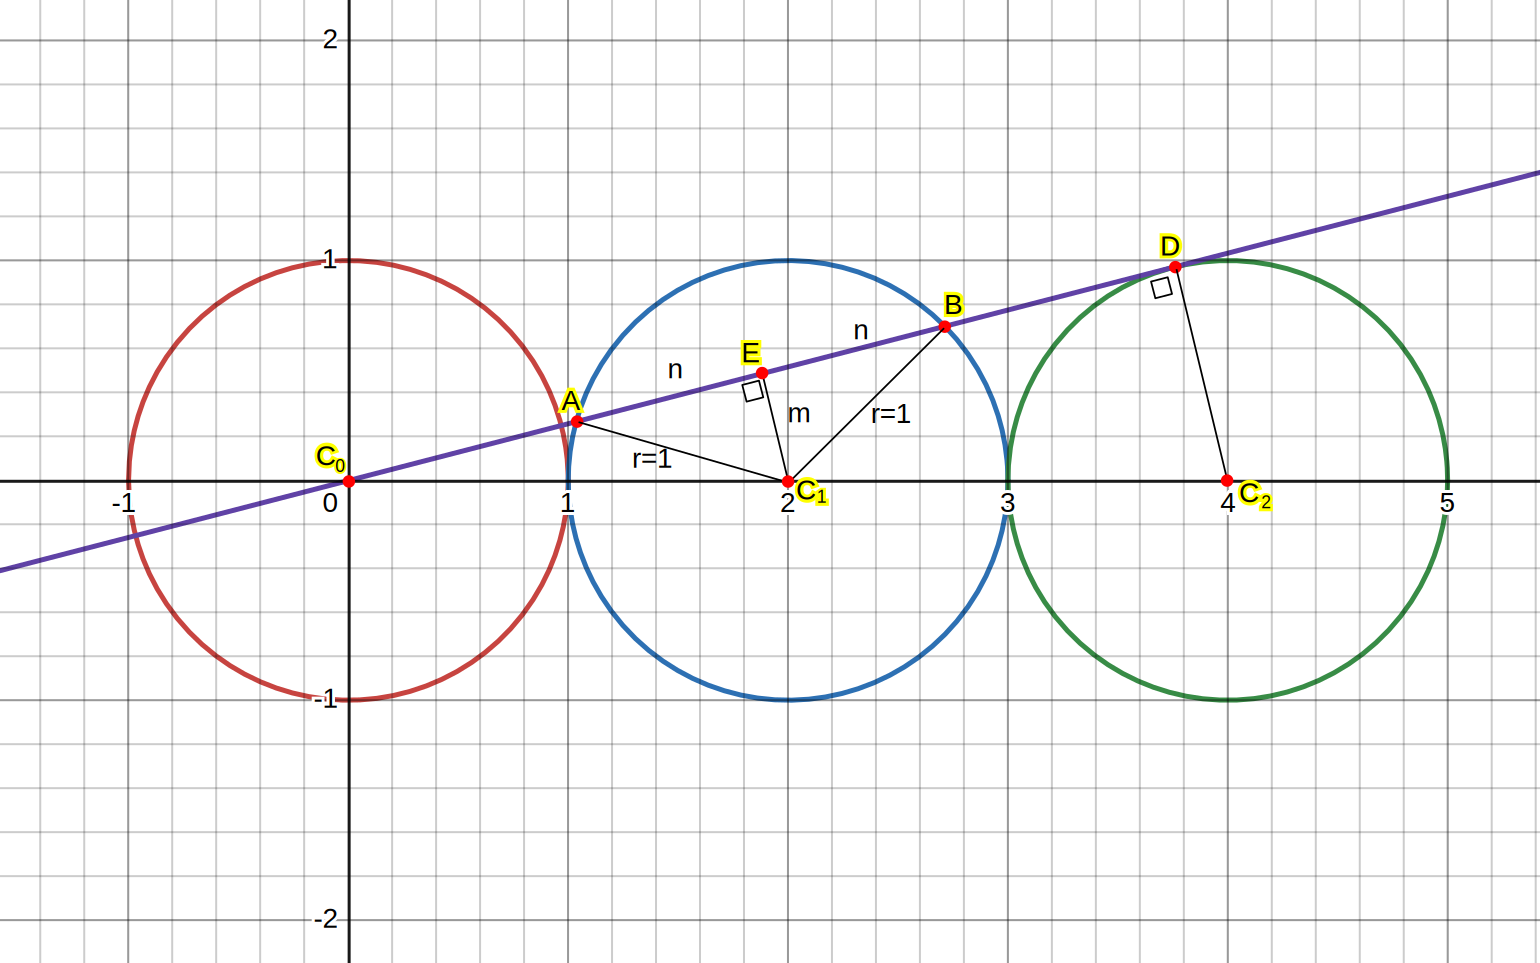
\includegraphics[width=0.8\textwidth]{circ_08_02.pdf}
\end{figure}

Il triangolo $\triangle{ABC_1}$ è isoscele in quanto i lati $\overline{AC_1}$ e
$\overline{BC_1}$ sono entrambi definiti 
dal raggio del cerchio che è uguale a $1$.

Dal punto $C1$ si traccia una perpendicolare al segmento $\overline{AB}$, che lo divide 
in due parti uguali di lunghezza $n=\frac{AB}{2}$.

Il punto $D$ è tangente al cerchio centrato in $(4,0)$ per cui l'angolo $\angle{BDC}$ è retto.

I due segmenti $\overline{EC_1}$ e $\overline{DC_2}$ sono paralleli in quanto perpendicolari alla stessa retta.

Gli angoli $\angle{C_0C_1E}$ e $\angle{C_0C_2D}$ sono uguali in quanto definiti da due rette parallele
che ne intersecano una terza.

I due triangoli $\triangle{C_0EC_1}$ e $\triangle{C_0DC_2}$ sono quindi simili; possiamo quindi scrivere 
una proporzione:

\[ \frac{\overline{C_0C_2}}{\overline{C_0C_1}} = \frac{\overline{DC_2}}{\overline{EC_1}} \]
\[ \frac{4}{2} = \frac{1}{m} \]
\[ m=\frac{1}{2} \]

A questo punto per Pitagora:
\[ n=\sqrt{r^2-m^2} \]
\[ n=\sqrt{1-\left(\frac{1}{2}\right)^2} \]
\[ n=\sqrt{\frac{3}{4}}, \overline{AB}=\sqrt{3} \]





\vspace{1cm}
\hrule
\vspace{1cm}



